\documentclass[conference]{IEEEtran}
\usepackage[T1]{fontenc}
\usepackage{graphicx,booktabs,amsmath,cite,url}
\usepackage[hidelinks]{hyperref}

\begin{document}

\title{Does Low-Communication Training Survive Bad Networks? A Reproducible Study of DDP, DiLoCo and Hierarchical Aggregation over Emulated WAN Links}

\author{\IEEEauthorblockN{<<AUTHOR>>}
\IEEEauthorblockA{Independent Researcher}}

\maketitle

\begin{abstract}
Training neural networks across geographically distributed sites is limited by slow, lossy wide-area links. Low-communication methods such as DiLoCo synchronize rarely, and hierarchical schemes aggregate within regions before crossing the WAN. We present a reproducible, CPU-scale study that trains a small transformer language model with four workers in two emulated regions and compares synchronous data parallelism (DDP), DiLoCo, and a two-level hierarchical DiLoCo, each with FP32, INT8 or INT4 compression of everything that crosses the WAN. Synchronization rounds are measured over real TCP connections through a packet-level emulator with per-region full-duplex links, finite buffers and a 1500-byte MTU, under four WAN profiles from 100\,Mbit/s to 2\,Mbit/s with 1\% loss. With the same 40 WAN synchronizations, hierarchical DiLoCo reached a validation loss of <<hier50>> versus <<dil50>> for flat DiLoCo, and it also beat flat DiLoCo synchronizing five times as often (<<dil10>>). INT8 and INT4 compression changed final loss by at most <<max_comp_delta>>. DDP reached the best loss (<<ddp>>) but, on a 10\,Mbit/s link, would spend an estimated <<ddp_constrained_min>> minutes on 2,000 steps versus <<hier8_constrained_min>> minutes for hierarchical DiLoCo with INT8. A real four-process distributed run matched the simulation's validation loss to within <<val_match>>, and the wall-clock model underestimated its total run time by <<under32>>--<<under8>>\%. Code and data are released.
\end{abstract}

\begin{IEEEkeywords}
distributed training, low-communication training, DiLoCo, local SGD, hierarchical aggregation, gradient compression, network emulation
\end{IEEEkeywords}

\section{Introduction}
Data-parallel training synchronizes gradients after every step, which assumes datacenter interconnects. When compute is spread across regions or organizations connected by the public internet, this assumption fails: a single synchronization of a model's parameters can take seconds over a congested or lossy wide-area network (WAN). Low-communication methods address this. DiLoCo~\cite{diloco} lets each worker take hundreds of local optimizer steps and then averages ``pseudo-gradients'' with an outer Nesterov-momentum step, and it has been used to train models across continents~\cite{opendiloco,intellect1}. Hierarchical variants first aggregate inside a region over fast local links and send only one update per region over the WAN~\cite{halos,lin2020}.

Most evaluations of these methods run on large GPU clusters and model WAN effects analytically. This paper asks a narrower, reproducible question: \emph{under realistic packet-level WAN behavior, how do synchronous, low-communication and hierarchical training compare in time and model quality?} Our contributions are:
\begin{enumerate}
\item An open testbed that runs on a single 4-core machine: a small transformer trained by four workers in two regions, real TCP synchronization rounds, and a WAN emulator with per-region full-duplex links, drop-tail buffers and a realistic MTU.
\item A comparison of DDP, DiLoCo and two-level hierarchical DiLoCo with FP32, INT8 and INT4 compression across four WAN profiles, with tuned hyperparameters and two seeds per configuration.
\item The finding that, at equal WAN synchronization counts, hierarchical aggregation improves model quality, while 8- and 4-bit compression is nearly free.
\item An end-to-end validation with real distributed processes, and a description of emulation pitfalls (TCP Small Queues, loopback MTU) that can distort such studies, together with a check for TCP slow start after idle.
\end{enumerate}

\section{Related Work}
Local SGD and federated averaging~\cite{fedavg,stich2019} reduce communication by averaging models after several local steps. Lin et al.~\cite{lin2020} proposed hierarchical local SGD, which synchronizes frequently within groups and rarely across them. DiLoCo~\cite{diloco} combines many inner AdamW~\cite{adamw} steps with an outer Nesterov step~\cite{sutskever2013}. Streaming DiLoCo~\cite{streamingdiloco} synchronizes parameter fragments and overlaps communication with computation, and OpenDiLoCo~\cite{opendiloco} and INTELLECT-1~\cite{intellect1} demonstrated globally distributed training, the latter with INT8 pseudo-gradients. DeMo~\cite{demo} reduces communication by synchronizing only fast-moving momentum components. HALoS~\cite{halos} introduces hierarchical asynchronous local SGD for geo-distributed LLM training. Gradient compression has a long history, including 1-bit SGD~\cite{seide2014}, QSGD~\cite{qsgd} and deep gradient compression~\cite{dgc}. Our study differs in scale and emphasis: it is small enough to reproduce on a laptop-class CPU, and it measures synchronization over real TCP connections through a packet-level emulator.

\section{Method}
\subsection{Model, data and training}
The model is a GPT-style character-level transformer (3 layers, width 96, 4 heads, context 64; <<n_params>> parameters) trained on Tiny Shakespeare~\cite{charrnn} (90/10 train/validation split). Four workers each sample batches of 16 sequences from a disjoint contiguous shard of the training text, so their data distributions differ mildly. Every method runs 2,000 steps per worker with AdamW ($\beta=(0.9,0.95)$, weight decay 0.1, gradient clipping 1.0, 100 warm-up steps, cosine decay to 10\%). Validation loss is computed on a fixed set of 512 held-out sequences. Training is implemented in JAX~\cite{jax}; workers are simulated with vectorization, which is mathematically identical to separate machines.

\subsection{Synchronization strategies}
\textbf{DDP} averages gradients across the four workers after every step (2,000 synchronizations). \textbf{DiLoCo} with period $H$: every $H$ steps, each worker $i$ forms the pseudo-gradient $\Delta_i=\theta_g-\theta_i$, the average $\bar\Delta$ is applied to the global parameters $\theta_g$ with outer SGD with Nesterov momentum (momentum 0.9), and every worker restarts from $\theta_g$. Inner optimizer states remain local. \textbf{Hierarchical DiLoCo} groups the workers into two regions of two. Every $H_r$ steps, workers average their parameters within their region over the local link. Every $H_g$ steps, each region sends one pseudo-gradient over the WAN to a global DiLoCo outer step. We use $H_r=10$ and $H_g\in\{50,100\}$, compared with flat DiLoCo at $H\in\{10,50,100\}$.

\subsection{Compression}
Everything that crosses the WAN, both the uploaded pseudo-gradients and the averaged result sent back, is quantized blockwise (256 values per block, one FP32 scale each) to INT8 or INT4 with symmetric round-to-nearest. Payloads are <<kb32>>\,kB (FP32), <<kb8>>\,kB (INT8) and <<kb4>>\,kB (INT4). Local-link traffic in the hierarchical scheme is FP32.

\subsection{Hyperparameter tuning}
On seed 0 we swept the DDP learning rate over $\{1,2,4,8,16\}\times10^{-3}$, and the DiLoCo ($H$=50) inner and outer learning rates. The sweep was extended twice because the best values initially lay at the edge of the range. The final choices were <<ddp_lr>> for DDP, and <<dil_lr>> (inner) with <<dil_olr>> (outer) for DiLoCo; DDP's loss differed by only 0.0002 between $8\times10^{-3}$ and $1.6\times10^{-2}$. Hierarchical DiLoCo reuses DiLoCo's values without further tuning. Reported results use seeds 1 and 2.

\subsection{Network testbed}
Each region reaches a central coordinator over its own emulated WAN link, while workers reach their regional hub over an unimpaired local link. A userspace emulator built on Linux NFQUEUE gives each link two independent directions. Each direction serializes packets at the link rate, adds propagation delay, drops packets at random with the configured probability, and enforces a drop-tail buffer of one bandwidth-delay product. The loopback MTU is set to 1500 bytes during measurements, and TCP uses Linux defaults (CUBIC~\cite{cubic}). Table~\ref{tab:profiles} lists the WAN profiles. A synchronization round is timed from the moment workers start sending to the moment all workers hold the averaged result. Rounds are separated by 1\,s, so TCP slow start after idle applies, as it would between DiLoCo synchronizations. Because DDP synchronizes after every step, its rounds were also measured back to back (50\,ms gaps), so that TCP congestion windows stay open; these rounds were within <<b2b_diff>>\% of rounds with idle gaps.

\begin{table}[t]
\caption{WAN profiles (per direction of each region's link).}
\label{tab:profiles}
\centering\footnotesize
\begin{tabular}{@{}lccc@{}}
\toprule
Profile & Rate & One-way delay & Loss \\
\midrule
Regional & 100\,Mbit/s & 10\,ms & 0\% \\
Intercontinental & 50\,Mbit/s & 75\,ms & 0.1\% \\
Constrained & 10\,Mbit/s & 100\,ms & 0.5\% \\
Poor & 2\,Mbit/s & 150\,ms & 1\% \\
\bottomrule
\end{tabular}
\end{table}

\subsection{Wall-clock model and validation}
Because every strategy is synchronous, its convergence per step does not depend on the network. We therefore estimate training time as
\begin{equation}
T = S\,t_c + N_{\mathrm{WAN}}\,r_{\mathrm{WAN}} + N_{\mathrm{LAN}}\,r_{\mathrm{LAN}},
\end{equation}
where $S=2{,}000$ steps, $t_c=$\,<<tc_ms>>\,ms is the measured per-worker compute time per step (four processes, one core each), $N$ is the number of synchronizations of each kind, and $r$ is the measured median round time. To validate this decomposition, we ran DiLoCo ($H$=50, 300 steps) as four real worker processes and a coordinator exchanging real quantized payloads over the constrained profile, and compared the result with the simulation.

\section{Results}
\subsection{Model quality}
Table~\ref{tab:quality} and Fig.~\ref{fig:curves} summarize final validation loss. DDP reached <<ddp>>. With the same 40 WAN synchronizations, hierarchical DiLoCo (10/50) reached <<hier50>>, better than flat DiLoCo ($H$=50, <<dil50>>), and also better than flat DiLoCo synchronizing five times as often ($H$=10, <<dil10>>). The same ordering held at 20 WAN synchronizations (hierarchical 10/100: <<hier100>>; DiLoCo $H$=100: <<dil100>>). A likely explanation is that frequent, cheap intra-region averaging reduces the divergence between workers, so each regional pseudo-gradient is a better estimate of the shared update.

\begin{table}[t]
\caption{Final validation loss (mean of seeds 1 and 2; range in brackets) and number of WAN synchronizations.}
\label{tab:quality}
\centering\footnotesize\setlength{\tabcolsep}{3pt}
\begin{tabular}{@{}lrrc@{}}
\toprule
Configuration & WAN syncs & Loss & [min, max] \\
\midrule
<<TABLE_QUALITY>>
\bottomrule
\end{tabular}
\end{table}

\begin{figure}[t]
\centering
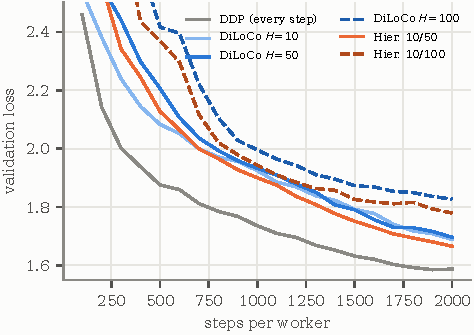
\includegraphics[width=\columnwidth]{figs/fig_curves.pdf}
\caption{Validation loss during training (FP32, mean of two seeds).}
\label{fig:curves}
\end{figure}

\subsection{Compression}
INT8 and INT4 quantization of WAN traffic changed final loss by at most <<max_comp_delta>> across the DiLoCo and hierarchical configurations, a difference comparable to the variation between seeds (Fig.~\ref{fig:comp}). Compression therefore cuts WAN bytes by 4--8$\times$ at little or no measurable cost at this scale.

\begin{figure}[t]
\centering
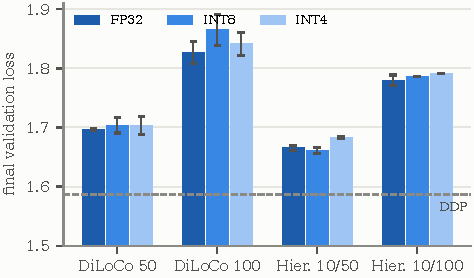
\includegraphics[width=\columnwidth]{figs/fig_compression.pdf}
\caption{Effect of WAN compression on final validation loss (bars: mean of two seeds; whiskers: range).}
\label{fig:comp}
\end{figure}

\subsection{Synchronization cost}
Table~\ref{tab:rounds} lists measured round times. Hierarchical aggregation roughly halves FP32 round time on the bandwidth-limited profiles (regional, constrained, poor), because each region link carries one update instead of two; on the latency-bound intercontinental profile the reduction is <<ic_hier_red>>\%. Compression helps most on low-bandwidth links. On high-latency links, rounds are dominated by round trips and TCP slow start rather than bytes: on the intercontinental profile, INT8 payloads are 4$\times$ smaller than FP32 but only about <<ic_ratio>>$\times$ faster.

\begin{table}[t]
\caption{Median synchronization round time in seconds (measured).}
\label{tab:rounds}
\centering\footnotesize\setlength{\tabcolsep}{3.5pt}
\begin{tabular}{@{}lrrrrrrr@{}}
\toprule
 & DDP & \multicolumn{3}{c}{Flat} & \multicolumn{3}{c}{Hierarchical} \\
\cmidrule(lr){2-2}\cmidrule(lr){3-5}\cmidrule(lr){6-8}
Profile & FP32 & FP32 & INT8 & INT4 & FP32 & INT8 & INT4 \\
\midrule
<<TABLE_ROUNDS>>
\bottomrule
\end{tabular}
\end{table}

\subsection{Time versus quality}
Fig.~\ref{fig:tq} combines quality and estimated training time. Computation alone takes <<compute_min>> minutes for 2,000 steps, so low-communication methods are close to compute-bound on all but the poor profile. DDP is the slowest on every profile, by a factor that grows as the network worsens: <<sp_regional>>$\times$ slower than hierarchical 10/50 with INT8 on the regional profile, <<sp_inter>>$\times$ on the intercontinental, <<sp_constrained>>$\times$ on the constrained (<<ddp_constrained_min>> versus <<hier8_constrained_min>> minutes) and <<sp_poor>>$\times$ on the poor profile (about <<ddp_poor_h>> hours versus <<hier8_poor_min>> minutes). Hierarchical 10/50 with INT8 has the second-best quality after DDP and lies on the time--quality frontier on all four profiles. DDP is preferable only when its quality advantage justifies its network cost.

\begin{figure*}[t]
\centering
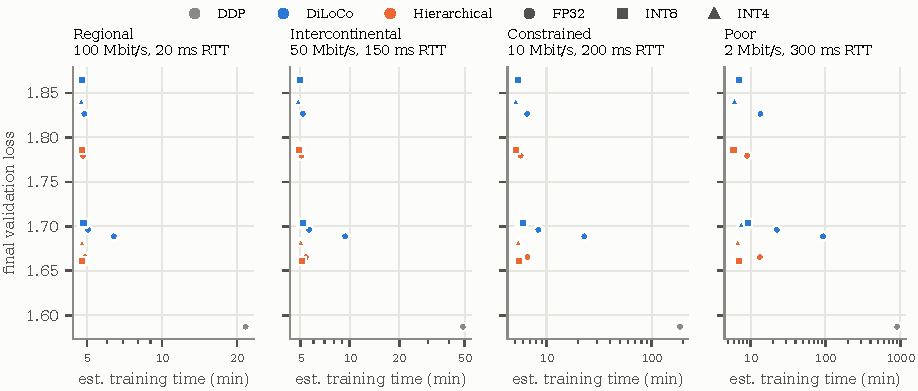
\includegraphics[width=\textwidth]{figs/fig_time_quality.pdf}
\caption{Estimated time for 2,000 steps (log scale) versus final validation loss for each configuration and WAN profile. Lower-left is better.}
\label{fig:tq}
\end{figure*}

\subsection{Validation}
The real four-process DiLoCo runs reached validation losses of <<dist32>> (FP32) and <<dist8>> (INT8), versus <<sim32>> and <<sim8>> in simulation (difference at most <<val_match>>). Their measured synchronization rounds had medians of <<dist_r32>>\,s (FP32) and <<dist_r8>>\,s (INT8), longer than the benchmark's <<bench_r32>>\,s and <<bench_r8>>\,s, because in real training workers enter a round at slightly different times and payloads must be encoded and decoded. As a result, the wall-clock model underestimated the real runs' total time by <<under32>>\% (FP32) and <<under8>>\% (INT8). These errors are small relative to the differences between methods, but the estimates in Fig.~\ref{fig:tq} should be read as lower bounds.

\section{Discussion and Limitations}
Several emulation details mattered. Queueing delayed packets on the sending side of loopback triggered TCP Small Queues and capped throughput at about 4\,Mbit/s on a 100\,Mbit/s link, so the emulator queues on the receive path. With loopback's default 64\,kB MTU, TCP would react far less to packet loss than on real paths~\cite{mathis1997}. We also measured DDP rounds back to back to rule out a penalty from TCP slow start after idle~\cite{rfc6928}; in our setting the effect was negligible.

The study is deliberately small: a 352K-parameter character-level model, 2,000 steps, four workers and two regions. The ratio of computation to communication differs from LLM training, where models are larger and steps slower, and DiLoCo has been reported to match synchronous training at larger scale~\cite{diloco}. Hyperparameters were tuned for DDP and flat DiLoCo, and the hierarchical scheme reused DiLoCo's values, so its advantage is not due to extra tuning. Local links were unimpaired, the WAN was emulated rather than real, and results are from two seeds.

\section{Conclusion}
Under realistic WAN behavior, synchronous data parallelism is dominated by communication. Hierarchical DiLoCo with INT8 compression reduced network time by <<net_min>>--<<net_max>>$\times$ relative to DDP across the four profiles, at a moderate quality cost. Hierarchical aggregation narrows that cost at no extra WAN traffic, and 8- or 4-bit compression is nearly free. Combining rare WAN synchronization, regional aggregation and compression is a practical recipe for training over bad networks.

\section*{Data Availability}
Code, raw results and the network emulator are available <<REPO_URL>>.

\section*{Acknowledgment}
The author used Claude (Anthropic), an AI assistant, to help write the code, run the experiments and draft this manuscript. The author is responsible for the content of the paper.

\bibliographystyle{IEEEtran}
\bibliography{refs}

\end{document}
